\documentclass[11pt, a4paper]{article}
\usepackage[utf8]{inputenc}
\usepackage[T1]{fontenc}
\usepackage[german]{babel}
\usepackage{geometry}
\usepackage{hyperref}
\usepackage{graphicx}
\usepackage{csquotes}
\usepackage{amsmath}

\geometry{a4paper, top=2.5cm, bottom=2.5cm, left=2.5cm, right=2.5cm}

\hypersetup{
    colorlinks=true,
    linkcolor=blue,
    filecolor=magenta,
    urlcolor=cyan,
    pdftitle={Ausarbeitung zum Pipeline-Architekturstil},
    pdfauthor={Dein Name}, % Passe dies an
    pdfsubject={Softwarearchitektur},
    pdfkeywords={Pipeline, Pipes and Filters, Architekturstil, Software Engineering},
    bookmarks=true,
    pdfpagemode=FullScreen,
}

\title{Ausarbeitung zum Pipeline-Architekturstil}
\author{Alber Jonas, Schweitzer Tim}
\date{\today}

\begin{document}

\maketitle

\begin{abstract}
\noindent Diese Ausarbeitung befasst sich mit dem Pipeline-Architekturstil, auch bekannt als Pipes-and-Filters-Architektur. Es werden die grundlegenden Konzepte, Komponenten und Funktionsweisen dieses Stils erläutert. Darauf aufbauend werden typische Anwendungsbereiche und konkrete Beispiele vorgestellt. Abschließend erfolgt eine kritische Bewertung der architektonischen Eigenschaften, indem die wesentlichen Vor- und Nachteile des Pipeline-Stils diskutiert werden. Die Darstellung basiert auf etablierten Quellen der Softwarearchitektur-Literatur.
\end{abstract}

\tableofcontents
\newpage

\section{Einführung und Kernkonzepte}

In der Welt der Softwarearchitektur existieren diverse etablierte Muster und Stile, die als Blaupausen für die Strukturierung von Softwaresystemen dienen. Einer dieser fundamentalen und weit verbreiteten Stile ist die Pipeline-Architektur, oft auch als Pipes-and-Filters-Architektur bezeichnet \cite{RichardsFord2020}. Dieser Stil entstand als natürliche Konsequenz der Modularisierung von Anwendungsfunktionalität in eigenständige Verarbeitungsschritte \cite{RichardsFord2020}. Seine Prinzipien sind vielen Entwicklern und Architekten intuitiv vertraut, insbesondere durch die Kommandozeilen-Interpreter von Unix-basierten Betriebssystemen wie Bash oder Zsh, wo Befehle über Pipes (`|`) miteinander verkettet werden \cite{RichardsFord2020}. Auch in der funktionalen Programmierung finden sich Parallelen, da viele Sprachelemente die Komposition von Funktionen fördern, was dem Konzept der Pipeline ähnelt \cite{RichardsFord2020}. Moderne Datenverarbeitungsparadigmen wie MapReduce bauen ebenfalls auf dieser Grundtopologie auf \cite{RichardsFord2020}. Es ist hervorzuheben, dass der Pipeline-Stil nicht auf Low-Level-Systemprogrammierung beschränkt ist, sondern ebenso effektiv für die Gestaltung komplexer Geschäftsanwendungen eingesetzt werden kann \cite{RichardsFord2020}.

Die Architektur basiert auf zwei zentralen Komponenten: \textbf{Filtern} (Filters) und \textbf{Pipes} \cite{RichardsFord2020}.

\subsection{Filter: Die Verarbeitungseinheiten}

Filter repräsentieren die aktiven Bausteine der Architektur, die für die eigentliche Datenverarbeitung zuständig sind \cite{RichardsFord2020}. Charakteristisch für Filter ist ihre Eigenständigkeit und Unabhängigkeit voneinander. Idealerweise sind sie zustandslos (`stateless`), was bedeutet, dass das Ergebnis einer Verarbeitung ausschließlich von den aktuellen Eingabedaten abhängt und nicht von vorherigen Interaktionen \cite{RichardsFord2020}. Ein Kernprinzip des Designs ist die \textit{Single Responsibility}: Jeder Filter sollte genau eine klar definierte Aufgabe erfüllen \cite{RichardsFord2020}. Steht eine komplexere Verarbeitungslogik an, wird diese nicht in einem einzigen, monolithischen Filter implementiert, sondern auf eine Sequenz spezialisierter Filter verteilt, die nacheinander ausgeführt werden \cite{RichardsFord2020}. Diese Granularität fördert die Wiederverwendbarkeit und Testbarkeit der einzelnen Komponenten.

Innerhalb der Pipeline-Architektur unterscheidet man typischerweise vier Arten von Filtern \cite{RichardsFord2020}:

\begin{itemize}
    \item \textbf{Producer (Erzeuger oder Quelle):} Dieser Filtertyp steht am Anfang einer Pipeline und ist für die Generierung der initialen Daten verantwortlich. Er empfängt keine Daten von einem vorherigen Filter, sondern agiert als Datenquelle, z.B. durch Lesen aus einer Datei, einer Datenbank oder einem Netzwerk-Socket. Er wird daher auch als »Source« bezeichnet \cite{RichardsFord2020}.
    \item \textbf{Transformer (Umwandler):} Ein Transformer nimmt Daten von einer Pipe entgegen, führt eine Transformation darauf aus (z.B. Daten anreichern, Format ändern, Werte berechnen) und leitet das modifizierte Ergebnis an die nächste Pipe weiter. Dieser Filtertyp verkörpert das zentrale Verarbeitungselement in vielen Pipelines. Funktionale Programmierer erkennen hier eine Analogie zur `map`-Operation \cite{RichardsFord2020}.
    \item \textbf{Tester (Filter im engeren Sinne):} Dieser Filter empfängt ebenfalls Daten, prüft diese jedoch anhand bestimmter Kriterien. Abhängig vom Ergebnis dieser Prüfung leitet er die Daten entweder unverändert weiter, verwirft sie oder leitet sie möglicherweise auf unterschiedliche Ausgänge (obwohl dies die klassische lineare Pipeline erweitert). Er selektiert also Datenströme. Funktionale Programmierer mögen hier an `filter`- oder `reduce`-Operationen denken, je nach spezifischer Implementierung \cite{RichardsFord2020}.
    \item \textbf{Consumer (Verbraucher oder Senke):} Der Consumer bildet das Ende einer Pipeline. Er nimmt die final verarbeiteten Daten entgegen und führt eine abschließende Aktion durch, wie das Speichern der Daten in einer Datenbank, das Anzeigen auf einer Benutzeroberfläche oder das Senden an ein externes System. Er wird auch als »Sink« bezeichnet \cite{RichardsFord2020}.
\end{itemize}

\subsection{Pipes: Die Kommunikationskanäle}

Pipes stellen die Verbindungen zwischen den Filtern dar und definieren den Datenfluss durch die Architektur \cite{RichardsFord2020}. Sie fungieren als gerichtete Kommunikationskanäle, die typischerweise genau einen Filterausgang mit genau einem Filtereingang verbinden (Punkt-zu-Punkt-Verbindung). Dies unterscheidet sie von Broadcast-Mechanismen, bei denen Daten an mehrere Empfänger gleichzeitig gesendet werden, was in der Regel aus Performancegründen vermieden wird \cite{RichardsFord2020}. Eine Pipe nimmt die Ausgabe eines Filters entgegen und leitet sie als Eingabe an den nächsten Filter weiter \cite{RichardsFord2020}.

Die Daten, die als Nutzlast (`payload`) durch die Pipes transportiert werden, können prinzipiell jedes beliebige Format haben – von einfachen Textströmen über strukturierte Daten wie XML oder JSON bis hin zu binären Objekten \cite{RichardsFord2020}. Für eine hohe Performance und geringe Kopplung zwischen den Filtern wird jedoch oft empfohlen, das Datenformat möglichst standardisiert und die Datenmenge pro Nachricht relativ klein zu halten \cite{RichardsFord2020}. Die Implementierung von Pipes kann vielfältig sein: von einfachen In-Memory-Warteschlangen in monolithischen Anwendungen bis hin zu komplexeren Message-Queues oder Netzwerkprotokollen in verteilten Systemen.

\subsection{Stärke durch Komposition: Das Unix-Beispiel}

Die wahre Stärke der Pipeline-Architektur liegt in der Komposition einfacher, wiederverwendbarer Bausteine zu komplexen Verarbeitungsketten. Die Unidirektionalität der Pipes und die Fokussierung der Filter auf einzelne Aufgaben machen sie hochgradig modular und wiederverwendbar \cite{RichardsFord2020}. Dieses Prinzip ist vielen Entwicklern aus der Unix-Shell-Nutzung bestens bekannt \cite{RichardsFord2020}.

Eine oft zitierte Anekdote illustriert eindrucksvoll die Eleganz und Mächtigkeit dieses Ansatzes \cite{RichardsFord2020}: Donald Knuth, ein renommierter Informatiker, wurde einst gebeten, ein Programm zu schreiben, das eine Textdatei einliest, die $n$ häufigsten Wörter identifiziert und diese zusammen mit ihrer Häufigkeit sortiert ausgibt. Sein Ergebnis war ein über zehn Seiten langes, dokumentiertes Pascal-Programm, das einen eigens entwickelten Algorithmus implementierte \cite{RichardsFord2020}. Doug McIlroy, einer der Väter von Unix und Pipes, präsentierte daraufhin eine Lösung als einfaches Shell-Skript, das dieselbe Aufgabe löste – wesentlich kürzer, verständlicher und oft sogar performanter. Dieses Skript, das problemlos in eine kurze Nachricht passt, lautete:
\begin{quote}
\texttt{tr -cs A-Za-z '\\textbackslash{}n' < input.txt | tr A-Z a-z | sort | uniq -c | sort -rn | head -n \$\{1:-10\}}
\end{quote}
Hierbei wird der Text zunächst in einzelne Wörter zerlegt (`tr`), in Kleinbuchstaben umgewandelt (`tr`), alphabetisch sortiert (`sort`), Duplikate gezählt (`uniq -c`), nach Häufigkeit numerisch und absteigend sortiert (`sort -rn`) und schließlich die ersten $n$ (hier standardmäßig 10) Zeilen ausgegeben (`head`). Jeder Befehl ist ein Filter, das Pipe-Symbol `|` repräsentiert die Pipe. Dieses Beispiel zeigt, wie mächtig die Kombination einfacher Werkzeuge sein kann, eine Komplexität, die selbst die Unix-Erfinder manchmal überraschte \cite{RichardsFord2020}.

\section{Anwendungsbereiche und Beispiele}

Der Pipeline-Architekturstil ist aufgrund seiner Struktur und Eigenschaften für eine Vielzahl von Anwendungsfällen prädestiniert. Insbesondere eignet er sich hervorragend für Systeme, die eine sequentielle, unidirektionale Verarbeitung von Datenströmen erfordern \cite{RichardsFord2020}. Die klare Trennung der Verarbeitungsschritte und der definierte Datenfluss machen ihn robust und nachvollziehbar für bestimmte Problemklassen.

Typische Anwendungsbereiche umfassen \cite{RichardsFord2020}:

\begin{itemize}
    \item \textbf{Elektronischer Datenaustausch (EDI):} Im Bereich EDI müssen oft Daten zwischen verschiedenen Formaten (z.B. unternehmensspezifische Formate, Industriestandards wie EDIFACT oder XML-Derivate) konvertiert werden. Pipeline-basierte Werkzeuge zerlegen diesen Prozess in Schritte wie Validierung, Mapping, Anreicherung und Formatkonvertierung, wobei jeder Schritt von einem spezialisierten Filter durchgeführt wird.
    \item \textbf{ETL-Prozesse (Extract, Transform, Load):} ETL-Werkzeuge, die Daten aus Quellsystemen extrahieren, transformieren und in Zielsysteme (oft Data Warehouses) laden, nutzen inhärent das Pipeline-Muster. Die Phasen Extraktion (Producer), Transformation (mehrere Transformer und Tester) und Laden (Consumer) bilden eine natürliche Pipeline. Die Architektur unterstützt hierbei sowohl den Datenfluss als auch die schrittweise Modifikation der Daten.
    \item \textbf{Orchestrierung und Mediation in Integrationsszenarien:} Werkzeuge wie Apache Camel oder Mule ESB verwenden oft Pipeline-Konzepte, um komplexe Integrationsprozesse und Geschäftsworkflows zu modellieren. Nachrichten oder Datenobjekte werden durch eine Kette von Verarbeitungsschritten (z.B. Protokolltransformation, Routing, Inhaltsanreicherung) geleitet, die als Filter in einer Pipeline konfiguriert sind.
    \item \textbf{Compiler-Konstruktion:} Klassische Compiler arbeiten oft nach einem Pipeline-Prinzip: Lexikalische Analyse -> Syntaktische Analyse -> Semantische Analyse -> Zwischencode-Erzeugung -> Optimierung -> Zielcode-Erzeugung. Jede Phase nimmt die Ausgabe der vorherigen als Eingabe und führt eine spezifische Transformation durch.
    \item \textbf{Verarbeitung von Streaming-Daten:} Systeme, die kontinuierliche Datenströme verarbeiten (z.B. Sensordaten, Log-Events, Finanztransaktionen), setzen häufig Pipelines ein. Frameworks wie Apache Kafka Streams, Flink oder Spark Streaming ermöglichen die Definition von Verarbeitungstopologien, die dem Pipes-and-Filters-Modell folgen.
\end{itemize}

\subsection{Beispiel: Verarbeitung von Telemetriedaten mit Kafka}

Ein anschauliches Beispiel für die Anwendung der Pipeline-Architektur ist die Verarbeitung von Telemetriedaten, die von verteilten Diensten erzeugt und über Apache Kafka gestreamt werden \cite{RichardsFord2020}. Ziel könnte sein, aus dem rohen Datenstrom spezifische Metriken wie Antwortzeiten und Verfügbarkeit zu extrahieren und zu aggregieren.

Eine mögliche Pipeline könnte wie folgt aufgebaut sein \cite{RichardsFord2020}:

1.  \textbf{Producer (`ServiceInfoCapture`):} Dieser Filter abonniert das relevante Kafka-Topic, in das die Rohdaten der Telemetrie (z.B. Logs oder Ereignisse über Serviceaufrufe) geschrieben werden. Er fungiert als Quelle der Pipeline und liest die Nachrichten aus Kafka.
2.  \textbf{Tester (`DurationFilter`):} Die vom Producer gelesenen Daten werden an diesen Filter weitergeleitet. Seine Aufgabe ist es zu prüfen, ob die aktuelle Nachricht Informationen über die Dauer (Antwortzeit) eines Serviceaufrufs enthält (z.B. einen Messwert in Millisekunden). Dies illustriert die klare Trennung: Der `ServiceInfoCapture`-Filter kümmert sich nur um das Lesen aus Kafka, der `DurationFilter` nur um die Identifikation relevanter Daten für diesen Zweig der Verarbeitung.
3.  \textbf{Transformer (`DurationCalculator`):} Wenn der `DurationFilter` feststellt, dass die Daten die Antwortzeit betreffen, leitet er sie an diesen Filter weiter. Der `DurationCalculator` könnte beispielsweise die Zeit von Millisekunden in Sekunden umrechnen, statistische Berechnungen durchführen (z.B. gleitender Durchschnitt) oder die Daten für die spätere Aggregation vorbereiten.
4.  \textbf{Tester (`UptimeFilter`):} Falls der `DurationFilter` die Nachricht nicht als relevant für die Antwortzeit einstuft, könnte sie alternativ an den `UptimeFilter` geleitet werden. Dieser prüft, ob die Nachricht stattdessen Informationen zur Verfügbarkeit oder zum Betriebsstatus des Dienstes enthält (z.B. Heartbeat-Signale, Fehlermeldungen).
5.  \textbf{Transformer (`UptimeCalculator`):} Wenn der `UptimeFilter` Uptime-relevante Daten erkennt, werden diese an den `UptimeCalculator` übergeben. Dieser Filter könnte den Status interpretieren und daraus Verfügbarkeitsmetriken ableiten (z.B. Berechnung der Uptime-Prozentrate über ein Zeitfenster).
6.  \textbf{Consumer (`DatabaseOutput` oder `MetricsAggregator`):} Die von `DurationCalculator` oder `UptimeCalculator` transformierten Metrikdaten werden schließlich an einen oder mehrere Consumer übergeben. Ein `DatabaseOutput`-Filter könnte die berechneten Metriken in einer Zeitreihendatenbank (z.B. InfluxDB, MongoDB) speichern \cite{RichardsFord2020}. Ein anderer Consumer könnte die Metriken an ein Monitoring-System weiterleiten.

Daten, die weder vom `DurationFilter` noch vom `UptimeFilter` als relevant eingestuft werden, verlassen die Pipeline an dieser Stelle, da sie für den spezifischen Zweck dieser Verarbeitungskette nicht benötigt werden \cite{RichardsFord2020}. Dieses Beispiel demonstriert, wie durch die Kombination verschiedener Filtertypen ein komplexer Verarbeitungsworkflow strukturiert werden kann, wobei jeder Filter eine klar umrissene Aufgabe übernimmt und der Datenfluss explizit durch die Pipes definiert ist.

\section{Bewertung: Vor- und Nachteile}

Wie jeder Architekturstil weist auch die Pipeline-Architektur spezifische Stärken und Schwächen auf, die bei der Entscheidung für oder gegen ihre Anwendung in einem konkreten Projektkontext abgewogen werden müssen. Die Bewertung erfolgt anhand gängiger architektonischer Qualitätsmerkmale \cite{RichardsFord2020}.

\subsection{Vorteile}

Die Pipeline-Architektur bietet eine Reihe signifikanter Vorteile, die sie für bestimmte Anwendungsfälle attraktiv machen:

\begin{itemize}
    \item \textbf{Einfachheit und Verständlichkeit:} Der lineare Datenfluss und die klare Aufgabentrennung der Filter machen die Architektur relativ einfach zu verstehen und nachzuvollziehen. Dies reduziert die kognitive Last für Entwickler und erleichtert die Einarbeitung neuer Teammitglieder \cite{RichardsFord2020}.
    \item \textbf{Modularität und Wiederverwendbarkeit:} Filter sind per Definition unabhängige Einheiten mit einer spezifischen Aufgabe. Sie können oft ohne Modifikation in verschiedenen Pipelines wiederverwendet werden. Die lose Kopplung über die Pipes erlaubt es, Filter auszutauschen, neu anzuordnen oder hinzuzufügen, ohne andere Filter direkt zu beeinflussen \cite{RichardsFord2020}. Dies fördert die Wartbarkeit und Flexibilität des Systems.
    \item \textbf{Technische Partitionierung:} Die Logik der Anwendung ist klar entlang der technischen Verarbeitungsschritte (Filtertypen wie Producer, Transformer, Tester, Consumer) aufgeteilt. Dies unterstützt eine strukturierte Entwicklung \cite{RichardsFord2020}.
    \item \textbf{Flexibilität bei der Komposition:} Die Möglichkeit, komplexe Aufgaben durch die Verkettung einfacher Filter zu lösen, bietet eine hohe Flexibilität im Design von Verarbeitungsprozessen. Neue Anforderungen können oft durch Hinzufügen oder Austauschen von Filtern implementiert werden.
    \item \textbf{Natürliche Parallelisierbarkeit (potenziell):} Obwohl oft monolithisch implementiert, bietet das Modell prinzipiell Potenzial für Parallelisierung. Einzelne Filterinstanzen könnten parallel arbeiten (Task-Parallelität), oder die Pipeline selbst könnte auf mehrere Datenströme parallel angewendet werden (Daten-Parallelität), sofern die Filter zustandslos sind und die Pipes dies unterstützen (z.B. durch konkurrente Queues).
    \item \textbf{Geringe Gesamtkosten (in bestimmten Szenarien):} Durch die Einfachheit, Verständlichkeit und Wiederverwendbarkeit können die Entwicklungs- und Wartungskosten, insbesondere für klar definierte sequentielle Prozesse, vergleichsweise niedrig sein \cite{RichardsFord2020}.
\end{itemize}

\subsection{Nachteile}

Trotz ihrer Vorteile bringt die Pipeline-Architektur auch einige Nachteile und Einschränkungen mit sich, die insbesondere bei komplexen oder hochskalierbaren Systemen relevant werden:

\begin{itemize}
    \item \textbf{Monolithisches Deployment (häufig):} In vielen Fällen wird eine Pipeline-Architektur als eine einzige Einheit (Monolith) bereitgestellt \cite{RichardsFord2020}. Das bedeutet, das gesamte System bildet ein einzelnes architektonisches Quantum. Änderungen an einem einzigen Filter erfordern potenziell das Testen und Deployen der gesamten Anwendung \cite{RichardsFord2020}.
    \item \textbf{Eingeschränkte Skalierbarkeit und Elastizität:} Aufgrund des typischerweise monolithischen Deployments ist die Skalierbarkeit oft auf die Skalierung der gesamten Anwendung beschränkt. Es ist schwierig, nur einzelne, ressourcenintensive Filter gezielt zu skalieren, ohne komplexe interne Mechanismen wie Threading oder asynchrone Verarbeitung einzuführen, für die der Stil nicht primär ausgelegt ist \cite{RichardsFord2020}. Die horizontale Skalierung des gesamten Monolithen kann ineffizient sein, wenn nur ein kleiner Teil der Pipeline der Flaschenhals ist. Dies führt zu einer niedrigen Bewertung bei Elastizität und Skalierbarkeit (oft nur ein Stern) \cite{RichardsFord2020}.
    \item \textbf{Geringe Fehlertoleranz und Verfügbarkeit:} In einer monolithischen Implementierung kann der Ausfall eines kritischen Filters (z.B. durch einen Fehler oder Ressourcenmangel wie Speicher) die gesamte Pipeline oder sogar die gesamte Anwendung zum Stillstand bringen \cite{RichardsFord2020}. Da es nur ein Deployment-Quantum gibt, fehlt die Isolation, die verteilte Systeme bieten. Die durchschnittliche Wiederherstellungszeit (MTTR) kann bei Monolithen relativ hoch sein (Minuten bis Stunden), was die Verfügbarkeit beeinträchtigt \cite{RichardsFord2020}.
    \item \textbf{Mittelmäßige Testbarkeit und Bereitstellbarkeit:} Obwohl einzelne Filter gut isoliert getestet werden können (Unit-Tests), erfordert jede Änderung am Code oft einen vollständigen Integrationstest und die erneute Bereitstellung des gesamten Monolithen. Dies verlangsamt den Entwicklungszyklus und erhöht das Risiko bei Deployments im Vergleich zu feingranulareren Architekturen wie Microservices \cite{RichardsFord2020}. Die Bewertung für Bereitstellbarkeit (`Deployability`) und Testbarkeit ist daher oft nur durchschnittlich \cite{RichardsFord2020}.
    \item \textbf{Potenzielle Latenzprobleme:} In langen Pipelines kann sich die Latenz summieren, da Daten sequenziell durch viele Filter fließen müssen. Wenn die Pipes zudem I/O-intensiv implementiert sind (z.B. über Festplatten-basierte Queues statt In-Memory), kann dies die End-to-End-Verzögerung weiter erhöhen.
    \item \textbf{Gemeinsames Datenformat als Herausforderung:} Die Notwendigkeit eines gemeinsamen Datenformats für die Pipes kann einschränkend sein oder zu Overhead führen, wenn Filter sehr unterschiedliche Datenrepräsentationen bevorzugen würden. Änderungen am Datenformat können Anpassungen in vielen Filtern erfordern.
    \item \textbf{Schwierigkeiten bei komplexen Kontrollflüssen:} Der Stil eignet sich am besten für lineare Abläufe. Komplexe Verzweigungen, Zusammenführungen oder iterative Prozesse können schwierig und unübersichtlich in einer reinen Pipeline-Struktur abzubilden sein.
\end{itemize}

\subsection{Fazit zur Bewertung}

Zusammenfassend lässt sich sagen, dass die Pipeline-Architektur ein eleganter und effektiver Stil für Probleme ist, die sich gut als sequentielle Kette von Verarbeitungsschritten modellieren lassen. Ihre Stärken liegen in der Einfachheit, Modularität und Wiederverwendbarkeit der Komponenten, was oft zu kosteneffizienten Lösungen führt \cite{RichardsFord2020}. Die größten Herausforderungen ergeben sich typischerweise aus der oft monolithischen Natur der Implementierung, was zu Einschränkungen bei Skalierbarkeit, Fehlertoleranz, Testbarkeit und Bereitstellbarkeit führt, insbesondere bei großen, komplexen oder hochverfügbaren Systemen \cite{RichardsFord2020}. Die Wahl dieses Stils sollte daher sorgfältig gegen die spezifischen Anforderungen des Systems abgewogen werden.

\section{Praktische Umsetzung: Beispiel einer Datenverarbeitungs-Pipeline}
\subsection{Gesamtarchitektur}
Um die Konzepte der Pipeline-Architektur zu verdeutlichen, betrachten wir im Folgenden eine beispielhafte Datenverarbeitungs-Pipeline. Diese Pipeline ist darauf ausgelegt, Sensordaten zu laden, zu verarbeiten und schließlich zu speichern. Der Startpunkt der Verarbeitung ist das Laden der Daten aus einer Datei.

Die grundlegende Architektur dieser Beispiel-Pipeline ist in Abbildung \ref{fig:architektur} schematisch dargestellt. Sie visualisiert den sequenziellen Fluss der Daten durch die einzelnen Verarbeitungsstufen.

\begin{figure}[htbp] % h: here, t: top, b: bottom, p: page of floats
    \centering % Center the image
    % Ersetzen Sie die folgende Zeile durch Ihren tatsächlichen \includegraphics-Befehl
    \fbox{\parbox[c][8cm][c]{0.9\textwidth}{\centering Platzhalter für Abbildung \texttt{img/architektur.png} \\ (Diagramm der Pipeline-Architektur)}}
    % Beispiel: \includegraphics[width=0.9\textwidth]{img/architektur.png}
    \caption{Schematische Darstellung der Datenverarbeitungs-Pipeline mit ihren Hauptstufen.} % Add a caption
    \label{fig:architektur} % Add a label for referencing
\end{figure}

Die Pipeline lässt sich in die folgenden logischen Stufen unterteilen, die nacheinander durchlaufen werden:

\begin{enumerate}
    \item \textbf{Datenerfassung (Laden):} In dieser ersten Stufe werden die Rohdaten von der Datenquelle (z.B. einer Sensordatei) eingelesen. Dies beinhaltet das Öffnen der Datei und das Parsen des Inhalts in eine interne Datenstruktur.
    \item \textbf{Vorverarbeitung:} Die geladenen Rohdaten werden bereinigt und gefiltert. Dies kann Schritte wie das Entfernen von Ausreißern, das Behandeln fehlender Werte oder das Glätten von Signalen umfassen.
    \item \textbf{Anreicherung:} Die vorverarbeiteten Daten werden mit zusätzlichen Kontextinformationen angereichert. Beispiele hierfür sind das Hinzufügen von Zeitstempeln, geografischen Koordinaten oder Metadaten zur Datenquelle.
    \item \textbf{Analyse:} In dieser Stufe erfolgt die eigentliche fachliche Verarbeitung. Dies kann spezifische Berechnungen, die Anwendung von Algorithmen zur Mustererkennung oder die Extraktion relevanter Merkmale beinhalten.
    \item \textbf{Speicherung/Ausgabe:} Die verarbeiteten Ergebnisse werden persistiert (z.B. in einer Datenbank oder Datei gespeichert) oder an nachfolgende Systeme zur weiteren Verwendung oder Visualisierung übergeben.
\end{enumerate}

Jede dieser Stufen repräsentiert eine logische Einheit innerhalb der Pipeline. Wie diese Stufen technisch implementiert und zu einer funktionierenden Pipeline zusammengesetzt werden, wird in den folgenden Abschnitten detailliert erläutert, beginnend mit der Implementierung der Pipeline-Steuerung.

\subsection{Implementierung der Pipeline-Steuerung: Die Wrapper-Klasse}
Nachdem die grundlegende Architektur und die einzelnen Stufen definiert sind, bedarf es einer Komponente, welche die Pipeline als Ganzes verwaltet und deren Ausführung steuert. Hierfür gibt es verschiedene Ansätze:

\begin{itemize}
    \item \textbf{Direkte Implementierung im Code:} Die Abfolge der Stufen wird direkt im ausführenden Code definiert. Dies ist einfach für kleine Pipelines, kann aber bei wachsender Komplexität unübersichtlich und schwer wartbar werden.
    \item \textbf{Konfigurationsbasierter Ansatz:} Die Pipeline-Struktur wird in einer externen Datei (z.B. YAML, JSON) definiert und zur Laufzeit geladen. Dies bietet hohe Flexibilität und ermöglicht Anpassungen ohne Code-Änderungen, erfordert jedoch zusätzlichen Aufwand für das Parsen und Validieren der Konfiguration.
    \item \textbf{Wrapper-Klasse:} Eine dedizierte Klasse kapselt die Logik zur Verwaltung der Stufen (Hinzufügen, Reihenfolge) und zur Ausführung der Pipeline. Dies fördert die Struktur, Kapselung und Wiederverwendbarkeit.
\end{itemize}

Für dieses Beispiel wird der Ansatz der Wrapper-Klasse gewählt, da er eine gute Balance zwischen Struktur, Flexibilität und Implementierungsaufwand bietet. Die Kernidee ist eine Klasse (z.B. `Pipeline`), die eine Liste von Pipeline-Stufen verwaltet und eine Methode zur Ausführung der gesamten Sequenz bereitstellt. Abbildung \ref{fig:wrapper} zeigt ein Klassendiagramm für eine solche Wrapper-Klasse.

\begin{figure}[htbp]
    \centering
    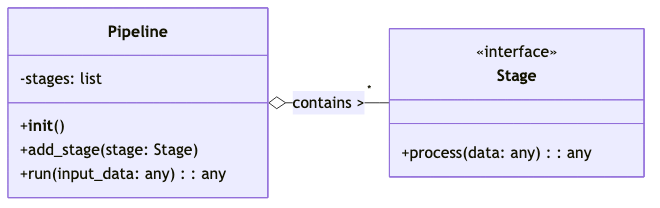
\includegraphics[width=0.8\textwidth]{img/wrapper.png}
    \caption{Klassendiagramm der Pipeline Wrapper-Klasse (`Pipeline`) und der abstrakten Stufenklasse (`Stage`).}
    \label{fig:wrapper}
\end{figure}

Die `Pipeline`-Klasse könnte typischerweise Methoden wie `\_\_init\_\_` (zur Initialisierung, z.B. einer leeren Liste für die Stufen), `add\_stage` (zum Hinzufügen einer Stufe zur Pipeline) und `execute` oder `run` (zum Durchlaufen aller Stufen mit den Eingabedaten) besitzen.

Ein zentrales Element dieses Ansatzes ist die Verwendung einer abstrakten Basisklasse oder einer Schnittstelle für die einzelnen Pipeline-Stufen (im Diagramm und folgenden Codebeispiel als `Stage` bezeichnet). Jede konkrete Stufe (wie Datenerfassung, Vorverarbeitung etc.) muss von dieser Basisklasse erben und deren definierte Methoden (z.B. eine `process` oder `execute`-Methode) implementieren. Dies stellt sicher, dass alle Stufen einheitlich behandelt und von der `Pipeline`-Klasse aufgerufen werden können.

Die Wrapper-Klasse kann zudem sicherstellen, dass nur valide Stufen hinzugefügt werden. Dies wird oft durch Typ-Prüfungen realisiert, wie im folgenden Python-Codeausschnitt für die `add\_stage`-Methode gezeigt:

\begin{verbatim}
# Innerhalb der Pipeline-Wrapper-Klasse
def add_stage(self, stage: Stage):
    """Fügt eine neue Stufe zur Pipeline hinzu."""
    if not isinstance(stage, Stage): # Prüft, ob das Objekt eine Instanz von Stage oder einer Subklasse ist
        raise TypeError("Übergebene Stufe muss eine Instanz von Stage sein.")
    self.stages.append(stage) # Annahme: self.stages ist die Liste der Stufen
\end{verbatim}

Diese Prüfung mittels `isinstance(stage, Stage)` stellt sicher, dass jedes Objekt, das der Pipeline hinzugefügt wird, tatsächlich vom Typ `Stage` (oder einer davon abgeleiteten Klasse) ist und somit die erwartete Schnittstelle (z.B. eine `process`-Methode) implementiert. Wird ein unpassendes Objekt übergeben, wird ein `TypeError` ausgelöst, was die Robustheit der Pipeline erhöht.

Die Kapselung der Pipeline-Logik in einer Wrapper-Klasse in Kombination mit einer abstrakten Basisklasse für die Stufen führt zu einem modularen, gut testbaren und erweiterbaren Design. Änderungen an einzelnen Stufen oder das Hinzufügen neuer Stufen beeinflussen die Wrapper-Klasse nur minimal, solange die definierte Schnittstelle eingehalten wird.

\begin{verbatim}
def add_stage(self, stage:Stage):
    if(not issubclass(stage, Stage)):
        raise TypeError("stage must be an instance of Stage")
\end{verbatim}\

Diese Sicherung wird in Python durch das Prüfen des Klassentyps (issubclass) sichergestellt. Wird eine Klasse übergeben welche keine Subklasse von Stage ist wird ein TypeError geworfen. Dies geschieht bei issubclass selbst bei einer erzeugten Instanz von Stage selbst.

\subsection{Factory Pattern zur dynamischen Komponentenauswahl}
Ein weiteres nützliches Entwurfsmuster, das häufig in Verbindung mit der Pipeline-Architektur eingesetzt wird, ist das Factory Pattern. Dieses Muster gehört zu den Erzeugungsmustern und dient dazu, Objekte zu erstellen, ohne die genaue Klasse des zu erstellenden Objekts im Voraus festlegen zu müssen. Stattdessen wird die Verantwortung für die Objekterzeugung an eine spezialisierte "Factory"-Klasse oder -Methode delegiert.

Das Factory Pattern ermöglicht eine signifikante Entkoppelung des aufrufenden Codes (in unserem Fall die Pipeline oder eine ihrer Stufen) von der konkreten Implementierung der zu erzeugenden Objekte. Die Factory fungiert als zentraler Punkt für die Erzeugung von Objekten eines bestimmten Typs oder einer bestimmten Schnittstelle. Abhängig von den übergebenen Parametern oder dem Kontext entscheidet die Factory, welche spezifische Unterklasse instanziiert und zurückgegeben werden soll.

\subsubsection{Anwendung im Datenlader}
In unserem Beispiel einer Datenverarbeitungs-Pipeline findet das Factory Pattern eine praktische Anwendung, insbesondere bei der Funktion zum Auslesen der Sensordateien. Unterschiedliche Sensoren oder Datenquellen können ihre Daten in verschiedenen Formaten bereitstellen (z.B. CSV, JSON, XML, Binärformate). Anstatt die Logik zur Erkennung und Verarbeitung jedes Formats direkt in die Pipeline-Stufe einzubetten, die die Daten lädt, wird eine `LoaderFactory` eingesetzt.

Der Ablauf ist typischerweise wie folgt:
\begin{enumerate}
    \item Eine vorherige Pipeline-Stufe oder der Initialaufruf übergibt den Dateipfad oder eine andere Kennung der zu ladenden Daten an die Stufe, die für das Laden zuständig ist.
    \item Diese Ladestufe delegiert die Erzeugung des passenden Ladeobjekts an die `LoaderFactory`. Sie übergibt dabei relevante Informationen, wie z.B. den Dateipfad oder explizit das Dateiformat.
    \item Die `LoaderFactory` analysiert die übergebenen Informationen (z.B. die Dateiendung wie `.csv` oder `.json`).
    \item Basierend auf dieser Analyse instanziiert die Factory ein konkretes Ladeobjekt (z.B. eine Instanz von `CsvLoader` oder `JsonLoader`), das eine gemeinsame Schnittstelle (z.B. `DataLoader`) implementiert.
    \item Die Factory gibt das erzeugte Ladeobjekt an die aufrufende Pipeline-Stufe zurück.
    \item Die Pipeline-Stufe verwendet nun das erhaltene Ladeobjekt, um die Daten zu laden, ohne die spezifische Implementierung des Laders kennen zu müssen. Sie interagiert nur über die definierte Schnittstelle (`DataLoader`).
\end{enumerate}

Abbildung \ref{fig:loaderFactory} illustriert diesen Entscheidungsprozess innerhalb der Factory. Die Factory prüft das angeforderte Format und wählt den entsprechenden Loader aus. Sollte kein passender Loader für das angeforderte Format registriert sein oder die Datei nicht existieren, wird typischerweise ein Fehler ausgelöst oder ein Null-Objekt zurückgegeben, um das Problem zu signalisieren.

\begin{figure}[htbp] % h: here, t: top, b: bottom, p: page of floats
    \centering % Center the image
    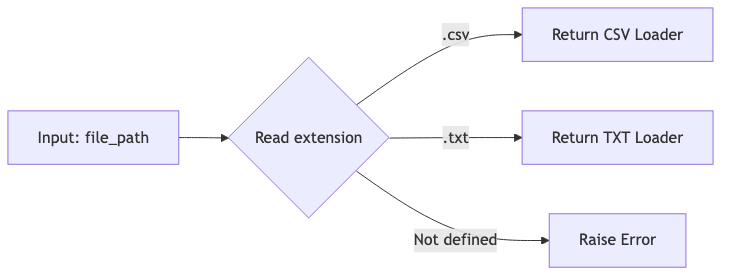
\includegraphics[width=0.8\textwidth]{img/LoaderFactory.png} % Include the image, adjust width as needed
    \caption{Entscheidungsdiagramm der LoaderFactory zur Auswahl des passenden Datenladers basierend auf dem Dateiformat.} % Add a caption
    \label{fig:loaderFactory} % Add a label for referencing
\end{figure}

\subsubsection{Vorteile des Factory Patterns in der Pipeline}
Der Einsatz des Factory Patterns in diesem Kontext bietet mehrere signifikante Vorteile:

\begin{itemize}
    \item \textbf{Entkoppelung:} Der Code der Pipeline-Stufe, die Daten lädt, ist von den konkreten Ladeimplementierungen entkoppelt. Er interagiert nur mit der Factory und der abstrakten `DataLoader`-Schnittstelle.
    \item \textbf{Flexibilität und Erweiterbarkeit (Open/Closed Principle):} Das Hinzufügen der Unterstützung für neue Dateiformate wird erheblich vereinfacht. Es muss lediglich eine neue `DataLoader`-Unterklasse (z.B. `XmlLoader`) implementiert und die `LoaderFactory` entsprechend erweitert werden, um diese neue Klasse bei Bedarf zu instanziieren. Der Code der Pipeline-Stufe selbst muss nicht modifiziert werden. Das System ist offen für Erweiterungen, aber geschlossen für Modifikationen.
    \item \textbf{Zentralisierung der Erzeugungslogik:} Die Logik zur Entscheidung, welcher Loader wann erstellt wird, ist an einem einzigen Ort – der Factory – konzentriert. Dies verbessert die Wartbarkeit und Übersichtlichkeit des Codes. Änderungen an der Erzeugungslogik müssen nur an dieser zentralen Stelle vorgenommen werden.
    \item \textbf{Verbesserte Testbarkeit:} Die einzelnen Loader-Klassen sowie die Factory selbst können isoliert getestet werden.
    \item \textbf{Wiederverwendbarkeit:} Die Factory und die Loader-Klassen können potenziell auch in anderen Teilen der Anwendung oder in anderen Projekten wiederverwendet werden. Wie bereits erwähnt, ist dies besonders nützlich, wenn die Ladefunktionalität als Teil eines wiederverwendbaren Moduls, Plugins oder Pakets (Pip Package) bereitgestellt wird. Entwickler, die das Paket nutzen, können eigene Loader hinzufügen und über die Factory registrieren (falls die Factory dies unterstützt), ohne den Kerncode des Pakets ändern zu müssen.
\end{itemize}

Zusammenfassend lässt sich sagen, dass das Factory Pattern die Struktur der Pipeline verbessert, indem es die Erzeugung von Komponenten wie Datenladern flexibler, wartbarer und erweiterbarer gestaltet. Es fördert ein sauberes Design, indem es Abhängigkeiten reduziert und Verantwortlichkeiten klar trennt.


\nocite{*}

\bibliographystyle{plain}
\bibliography{references} % Stellt sicher, dass die 'references.bib' Datei verwendet wird

\end{document}